\documentclass[10pt,conference]{IEEEtran}
\IEEEoverridecommandlockouts
% The preceding line is only needed to identify funding in the first footnote. If that is unneeded, please comment it out.
\usepackage{cite}
\usepackage{booktabs} % For formal tables
\usepackage{amsmath,amssymb,amsfonts}
\usepackage{algorithmic}
\usepackage{graphicx}
\usepackage{textcomp}
\usepackage{xcolor}
\usepackage{alltt}
\usepackage{ulem}
\def\BibTeX{{\rm B\kern-.05em{\sc i\kern-.025em b}\kern-.08em
    T\kern-.1667em\lower.7ex\hbox{E}\kern-.125emX}}
\begin{document}

\title{Cautious Adaptation of Defiant Components}

\author{\IEEEauthorblockN{1\textsuperscript{st} Given Name Surname}
\IEEEauthorblockA{\textit{dept. name of organization (of Aff.)} \\
\textit{name of organization (of Aff.)}\\
City, Country \\
email address}
\and
\IEEEauthorblockN{2\textsuperscript{nd} Given Name Surname}
\IEEEauthorblockA{\textit{dept. name of organization (of Aff.)} \\
\textit{name of organization (of Aff.)}\\
City, Country \\
email address}
\and
\IEEEauthorblockN{3\textsuperscript{rd} Given Name Surname}
\IEEEauthorblockA{\textit{dept. name of organization (of Aff.)} \\
\textit{name of organization (of Aff.)}\\
City, Country \\
email address}
\and
\IEEEauthorblockN{4\textsuperscript{th} Given Name Surname}
\IEEEauthorblockA{\textit{dept. name of organization (of Aff.)} \\
\textit{name of organization (of Aff.)}\\
City, Country \\
email address}
\and
\IEEEauthorblockN{5\textsuperscript{th} Given Name Surname}
\IEEEauthorblockA{\textit{dept. name of organization (of Aff.)} \\
\textit{name of organization (of Aff.)}\\
City, Country \\
email address}
\and
\IEEEauthorblockN{6\textsuperscript{th} Given Name Surname}
\IEEEauthorblockA{\textit{dept. name of organization (of Aff.)} \\
\textit{name of organization (of Aff.)}\\
City, Country \\
email address}
}

\maketitle

%\begin{abstract}
%Systems-of-systems are formed by the composition of independently created software components into a single system. Generally, the participating components are designed to satisfy their own requirements, and may not satisfy the overall requirements of the system-of-systems. We refer to components that cannot be adapted to meet both individual and global requirements as ``defiant" components. We then propose an adaptation approach that supports changing the behaviour of such defiant components under exceptional conditions. The approach uses scenarios to represent normal/ exceptional conditions, and models the behaviour of the exceptional conditions as wrappers implemented using an aspect-oriented technique. We refer to such adaptation as ``cautious", as it continues to guarantee the satisfaction of the original requirements of the components, while extending satisfaction to the exceptional conditions. We illustrate our approach and provide a preliminary evaluation of its feasibility using an organ delivery drone application.
%\end{abstract}

\begin{abstract}
Systems-of-systems are formed by the composition of independently created software components into a single system. These participating components are designed to satisfy their own requirements, and may not satisfy the overall requirements of the system-of-systems. We refer to components that cannot be adapted to meet both individual and global requirements as ``defiant" components. We propose a cautious adaptation approach that supports changing the behaviour of such defiant components under exceptional conditions to satisfy global requirements, while it continues to guarantee the satisfaction of the component's individual requirements. The approach uses scenarios to represent normal and exceptional conditions; models the behaviour of exceptional conditions as wrappers implemented using aspect-oriented technique; and executes runtime cautious adaptation. In the work, we consider both single and multiple defiant components, with several instances of these components operating at the same time. The implementation of the approach has been evaluated by using an organ delivery drone application. Results of the evaluation are presented and discussed in the paper. 
\end{abstract}

\begin{IEEEkeywords}
Defiant Component, Adaptation, Scenarios, Aspects 
\end{IEEEkeywords}

\section{Introduction}

\textit{It is now 10:00am in busy London. The kidney transplant department in St Thomas Hospital (Hospital A) has been informed that a matching kidney of a patient in Guy's Hospital (Hospital B) is now available for its patient waiting for surgery. The organ transplant department of both hospitals contact the SOSDronePayload company and make all the necessary arrangements for the organ to be transferred by drone from Hospital B to Hospital A. Drone\_DR1235 is selected by SOSDronePayload to deliver the organ through its flying corridor over the Thames River, to avoid land traffic. At a certain point during the journey the battery of Drone\_DR1235 reduces dramatically and when it reaches 10\%, Drone\_DR1235 attempts to land before reaching its final destination (Hospital A). However, at this point, Drone\_DR1235 was only 2 km away from Hospital A, 
% wind strong
and given the favourable wind conditions at the time, 
Drone\_DR1235 could have made the journey to Hospital A with its 10\% battery capacity and delivered the life critical organ.}

The above scenario is not unrealistic and likely to become increasingly common. In the scenario, \textit{Drone\_DR1235} was  developed independently of the payload organ delivery application, and was not intended to change its behaviour during its execution, regardless of the application in which it is used. 

Nowadays, many applications are developed by the composition of independently created software components into a single system. These systems are known as systems-of-systems~\cite{Maier98SOS} and allow the achievement of certain functionalities that cannot be achieved by individual participating components on their own.  In such situations, it is necessary to support emergent behaviours that appear due to the combination of existing components into new larger systems, or even due to new requirements or context changes ~\cite{SilvaSouza:2011:ARA:1988008.1988018}. The participating software components, however, have been designed to satisfy predefined requirements following predefined specifications and are not necessarily intended to change their behaviour during execution, nor to support some global requirements of the systems-of-systems applications. We refer to components that resist such changes, despite the need, as {\it defiant} components. 

Existing adaptation approaches have not considered such defiant components~\cite{filieri2011, DBLP:conf/dagstuhl/LemosGGGALSWBBB13, szvetits:2016, barbosa:2017, arcaini:2017}. In these approaches, models are often specified based on finite-state machine formalisms such as a labelled transition systems (LTS)~\cite{Magee:2006:CSM:1076396} or Markov chains~\cite{KNP11}, to represent system behaviour, verify property violation, and check the correctness of the adaptation. However, dealing with these models requires significant mathematical skills from the software engineers, which may hinder their adoption by users~\cite{barbosa:2017}. Such behaviour models also require a complete description of the system behaviour for a fixed scope and span~\cite{uchitel:2013}, which may not be possible for adaptive systems since not all adaptive behaviours can be modelled in advance due to unexpected requirements or environment uncertainty. 
 
In this paper we suggest a novel approach that considers the existence of defiant components. More specifically, we present a {\it cautious adaptation} approach in which changes in the behaviour of the components are acccomodated, in order to satisfy global requirements in exceptional circumstances. The adaptation is {\it cautious} as it guarantees that changes will not interfere with the original functionality of the participating components during their normal use, and will only be triggered in  exceptional conditions. For example, in the above scenario, the drone is considered a {\it defiant} component since it has been developed with a specification in which it should make a safe landing when its battery reaches 10\%. However, from the perspective of the payload organ delivery application, it should be possible to force the drone to continue flying, given the exceptional and favourable wind conditions, which will allow the drone to complete its journey.

Our approach relies on the use of {\it wrappers}, implemented using an aspect-oriented programming technique~\cite{Kiczales:2001}, to support exceptional conditions that are formalised with behavioural semantics using LTS~\cite{Magee:2006:CSM:1076396}. In our approach, exceptional conditions are represented by join-points of scenario-based aspect weaving~\cite{Xu07}, given that they can handle exceptions. The use of scenarios to identify exceptional conditions has been demonstrated successfully  in the literature~\cite{Young‐Gab:2011}\cite{Ban:2014}, and used to support behavioural model checking~\cite{uchitel:2003}. The high abstraction level provided by scenarios facilitates identification and understanding of requirements and involvement of different stakeholders in an application. The use of scenarios provides a framework for analysing future events of an application, by considering alternative situations, and helps with decision-making. 

The use of aspect-oriented programming  provides wrappers to support introducing changes into defiant components without requiring consent from the designer of the components. It avoids the need to redesign a component to satisfy emergent behaviours, as in the case when using, say,  dependency injection techniques~\cite{fowlerioc}  or plugin-based approaches~\cite{Wermelinger:2008:AEE:1370750.1370783}. On the other hand, the use of aspects-oriented programming techniques can be risky, since changes introduced by the use of aspects may violate the original (local) requirements of the components. Our work uses aspect-oriented techniques in a way that guarantees the original requirements of the components under normal execution conditions.  

The remainder of the paper is structured as follows. Section 2 describes our approach to support cautious adaptation of defiant components. Section 3 presents a running example of the payload organ delivery application. Section 4  discusses some conclusions and pointers to future work.



% Example
%Consider a system consists of Internet of Things (IoT) as an example. A person is running on an exercise machine and wearing a device that monitors the heartbeat rates. The person incrementally speeds up the machine, trying to test the limit. At a certain point, the wearable device alerts the person that the heart is beating very fast and something bad could happen. However, the runner does not listen to the advice and keeps increasing the machine speed (and, indirectly, his/her heart beating rate), thus putting the life in danger. Aware of the hazard, the wearable device connects to the training machine and stops it, against the runner's will.

%Consider an off-the-shelf drone that is designed to land safely when it cannot fly properly due to situations such as short of battery. This is a safety feature of commodity product where the software logic embedded in the controller firmware has been designed to satisfy a safety case properly. It is no longer safe any more, however, when the drone is being used for delivering a payload through the sky above water -- a legitimate medical use case to avoid traffic congestion in Central London when delivering emergency supply of blood and organs through a flight corridor on the Thames river. In the system perspective landing a drone on water is safer than landing it on someone's head or on a fast moving vehicle.

%For the drone flying above the river, the ``safe landing feature'' would drop the drone into water, losing a chance to achieve the system goal, i.e. to deliver the assets timely, because the sunk drone and payloads would require extra time to rescue. 

%In fact, the situation when it happens may not be all that pessimistic. If there is a bless of wind to add to the speed of
%the drone, and the remaining estimated time of arrival (ETA) is shorter than how long the drone can fly, a better recommendation for the drone is to fly on, overriding the internal condition to ``safe landing'' instruction set by the defiant component.

%While flying, the drone reports periodically to the pilot about its environment and internal status such as GPS locations and its battery levels. Suppose that the drone reports that its battery level is low and that it will not be able to land in the predefined place. Due to some internal failure or to an external interference (e.g., long distance from the pilot or bad weather conditions), the low-battery message does not reach the pilot, who keeps instructing the drone to fly forward. In this situation, the drone decides by itself to do a safe landing, since an out-of-battery failure could cause a  serious accident. However, as it is flying over a river (suppose the only allowed flight corridor in a big urban city), the drone may try to contact a ferry boat to rescue it, which has to decide whether it can help considering the distance and time of the probable drone landing place. In both examples, one of the components defies, either deliberately (e.g., the runner in the first example) or unintentionally (e.g., the pilot in the second example), to obey or accept messages from other component, thus putting at risk parts of the system and its surrounding environment. 

% Generalise the problem
%Although we have only described two possible scenarios, 
%The {\em defiant} problem may happen to various applications including cyber-physical systems, service-based systems, cyber security, system of systems, and cloud computing. The problem is challenging to predict at design time since each component has only local awareness of the system, restricted to its own behaviour model. However, when the components interact with each other at runtime, a global awareness of the system is needed where the interaction among the components cannot be anticipated at design time, due to the unpredictable human behaviour, possible component failures or on-the-fly intercommunication between a highly inter-operable and decoupled systems. Furthermore, the decisions about system conflict resolutions have been taken at design time.     

%% Solution requirements
%The solution to this ``defiant component'' problem needs a new type of software analysis approach, we call ``cautious adaptation'', wherein a {\em wrapper} of the defiant component is added so that (1) when the composed component does not exhibit defiant behaviour any more, without changing (tolerating) the defiant component at all; (2) the system shall satisfy the global safety goal, while relaxing the safety requirement of the defiant component in the exceptional scenarios. 

%% A solution
%What are our contributions
%As a contribution, we expect to improve the understanding of information modelling in runtime adaptive systems...  
%Given safety relaxation requirements and exceptional scenarios,
%there might be several ways to design the cautious adaptation wrappers. 

%In this paper, we propose one way to address this problem, by composing the defiant component and the wrapper through {\em decentralised dependency injection}. 

%% why dependency injection
%The proposed dependency injection inverses the control of dependencies between the defiant component and the wrapper function to satisfy the global goal in a situation that the component was not anticipating. Such cautious adaptation takes advantage of the situation awareness only known at the system level.

%% why decentralised
%Furthermore, the proposed solution is decentralised by design, because the wrapper may not be a single component. Indeed when dependence injector prepares the instantiation of the wrapper component incrementally, it is possible to distribute the wrapper functionality to several components. 

%% why cautious
%Built on top of established scenario-driven approach to behavioural model checking~\cite{uchitel2003}, we also introduce an exceptional scenario-driven approach to provide the needed assurance through model checking the {\em weakest safety property} of a defiant component. If such an optimistic assurance is not feasible, we degenerate the solution to a failure-responsive mode to reduce the risk to break an existing safety case which already governs the design of the defiant component.

%decides that the non-defiant component has to take over the system action control and try to leads the system to safe state. Such solution could have save real lives if, for instance, the plane that carried the Brazilian football team Chapecoense would have this solution implemented and, although the pilot insisted in keep flying, the airplane system would land it safely in the near airport, thus not running out of fuel.
%
%Some work have already proposed approaches for the dynamic composition of components, either in the cloud~\cite{Mathlouthi:2017}, in a service-based (eco)systems~\cite{Sun:2006}\cite{Cervantes:2014}, system of systems~\cite{Ricci:2012}, pervasive systems~\cite{Cervantes:2018}, they usually focus on engineering such composition or proposing new protocols, taking into account some non-functional requirements, such as performance, but do not address new safety requirements that arise for the new composed global system.   
%


% What are the challenges about this problem
%For that situation, some challenges arise as, for instance, how to model the system such that an early analysis of the risks can be carried out and, at the same time, propose a runtime adaptation to solve the conflict? For the best of our knowledge, no such approach for modelling the adaptation of the defiant component has been proposed.  

%Generally, to address behaviour adaptation, models are specified based on a finite-state machine formalism, such as a Labelled Transition System or Markov Chains, to represent the system behavior, verify property violation, and check the correctness of the adaptation\cite{filieri2011}\cite{bencomo2013}\cite{szvetits2016}\cite{barbosa2017}\cite{arcaini2017}. However, dealing with that kind of model demands a solid mathematical background by software engineers, which may hinder the adoption of such approaches for users who are not familiar with formal methods~\cite{barbosa2017}. Moreover, using such behaviour models requires a complete description of the system behaviour for a fixed scope and span~\cite{uchitel2013}, which may not be possible for a self-adaptive system since not all possible adaptive behaviours be modelled in advance due to unexpected changing requirements or environment uncertainty. 

% literature on scenarios
%In this realm, scenarios emerge as an alternative to model the expected (design time) and desired (run time) behaviours~\cite{uchitel2003}. Scenarios are a widespread modelling technique that, due to their high level of abstraction, eases the comprehension of requirements and the involvement of different stakeholders and provides a framework for analysing possible future events by considering alternative possible situations, thus helping the decision-making task. A scenario often refers to a partial description of the interaction between users, system components, and the environment in the restricted context of achieving some implicit purpose(s). The term \textit{partial} means that scenarios decompose complex system behaviour into smaller ``stories'' that are easy to understand and that, when combined with other scenarios, provide an overall system description. Each partial story typically focuses on different system functionalities

%More specifically, scenarios have been used successfully for security risk analysis and evaluation~\cite{Young‐Gab:2011}\cite{Ban:2014}.  

% what is our solution proposal
% why decentralized?
%In this paper, we propose a scenario-driven adaptation approach to model and resolve runtime conflicts regarding a defiant component. We use a Message Sequence Chart to model the scenarios and extend them with a special operator to indicate when a problem can take place. 



%\section{Background}

\subsection{Message Sequence Charts}


\subsection{Aspect-oriented Programming}

Aspect-oriented Programming (AOP)~\cite{Kiczales:2001} is a solution  to  address  problems  related  to  crosscutting  concerns   and   introduces   a   new   abstraction,   called   \textit{aspect} (which encapsulates typical AOP structures, i.e. joinpoints, pointcuts, advices and intertype declaraions),   as   well   as   a   flexible   mechanism   to   compose   aspects   with   object-oriented   components,   such  as  classes,  methods  and  attributes,  in  a  variety  of  ways.  Therefore,  this  new  paradigm  offers  means  to  separate  concerns  and,  consequently,  to  ensure  better  modularization.  %One  of  the  first  and  most  commonly  used AOP languages is AspectJ [2], which, as we have mentioned previously, is a direct extension of the Java programming language. For a more in-depth discussion about  AspectJ,  and  AOP  in  general,  the  reader  can  refer to [2]. 

%%\section{Cautious Adaptation Approach}
%Our approach to cautious adaptation of a defiant component is explained below.



\subsection{Motivating example}

Returning to the example mentioned in the introduction, Figure~\ref{fig:drone_msc} shows high-level message sequence charts (hMSC) specification for the delivery medical payload scenario. Each box in the hMSC corresponds to a basic message sequence chart (bMSC), like UML sequence diagrams, exchanging messages between different entities, while the bMSC are put together through control flows (branches and loops). Figure~\ref{fig:drone_bmsc} depicts the bMSC for the drone delivery example.   
% Need one example bMSC. 

\begin{figure}
    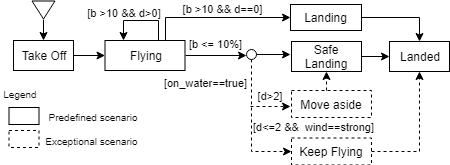
\includegraphics[scale=0.55]{figures/new_drone_msc.png}
    \caption{hMSCs for the drone scenario}
    \label{fig:drone_msc}
\end{figure}

\begin{figure}
    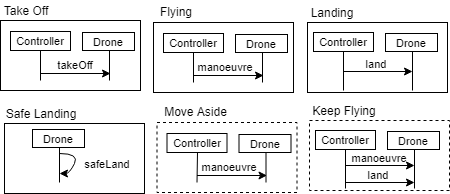
\includegraphics[scale=0.5]{figures/new_drone_bmsc.png}
    \caption{bMSCs for the drone delivery scenario}
    \label{fig:drone_bmsc}
\end{figure}

In the hMSC of Figure~\ref{fig:drone_msc}, the pre-defined scenarios, represented by a full rectangle, are part of the normal specification of the drone. Thus, the pilot, via a controller, can make the drone taking off, then keeps manoeuvring it where the battery is above the threshold $\theta = 10\%$  and it does not reach the expected location. When it does, then the pilot send a landing command to the drone, which acknowledge when landed in the ground.  During the flight, the drone periodically checks the status of its internal components, such as battery level and distance from the destination, represented by \textit{b} and \textit{d}, respectively, in the conditions over the hMSC transitions. In the example, if the battery level is below the threshold, then the drone reports the controller its data, otherwise it performs a safe landing by itself, since this is according to its predefined specification. 

However, the pilot knows that, if the distance from the expected landing pad is less than 1km and the drone is flying over the river (condition \textit{on\_water==true}), then he/she can keep the drone flying even in a low-level battery situation and then land it, thus being able to complete its overall goal (delivering the medical payload) successfully. Nonetheless, if the battery is low, the drone is above water, but the drone is more than 2km away, then necessary action is to move the drone aside in order to make it land on the ground. We represent those exceptional scenarios graphically by a dashed rectangle.  

We extend the MSC specification with the operator (o), which represents an \textit{interception point} in which exceptional scenarios can be plugged in to enable  wrapping the defiant behaviour of the drone. Note that more exceptional behaviours could be plugged in the same injection point indicating another possible behaviours according to other contextual information. If there is no exceptional scenario plugged in the injection point, then the expected behaviour is performed.

%In order to analyse this strategy, we transform the scenario specification into LTS models for each component, and then compose them in parallel to obtain the global behaviour of the system, as in~\cite{Uchitel:2003}. To do so, we need to introduce a special internal transition to represent the late decision on what would be the runtime behaviour of the defiant component. For instance, the first model shown in Figure~\ref{fig:drone_lts} (CONTROLLER\textunderscore DRONE) illustrates the LTS for the composition of the drone and the controller components in which a transition called \textit{decision} is introduced (from state 5 to 6) to indicate the injection point. See that, the next action after \textit{decision} is \textit{safeLanding}, i.e., if no exceptional scenario is plugged, then the component follows its ordinary behaviour.    

%The second model of Figure~\ref{fig:drone_lts} represents the model of the exceptional scenario, which we called as WRAPPER. Note that it contains the \textit{decision} action to synchronize with the its counterpart in the previous model, but after \textit{decision} is reached, the Wrapper changes the behaviour to keep the drone flying and, after, landing. This can be seen in the composition model of the system (controller and drone) and the wrapper, which is represented by model S in Figure~\ref{fig:drone_lts}. Therefore, the composition with the wrapper avoided the drone of performing its defiant behaviour.    

%\begin{figure}
%    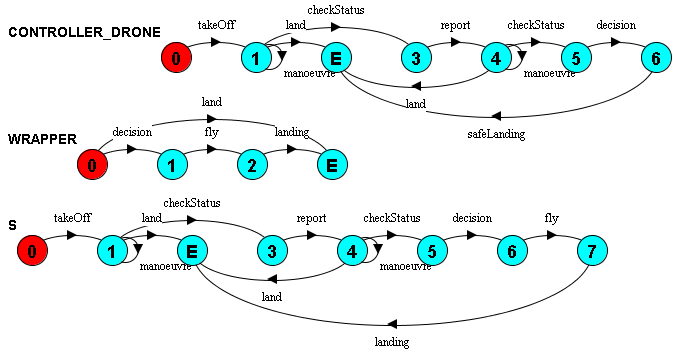
\includegraphics[scale=0.55]{figures/wrapper_lts.png}
%   \caption{LTS behaviour for drone and wrapper components }
%    \label{fig:drone_lts}
%\end{figure}


%!TEX root=main.tex
\section{Cautious Adaptation Approach}

Given a component that does not satisfy the global requirements of a system, although it is necessary to use the component. We call this component {\em defiant} if it can still be modified by adapting the system wrapping around it. In general, when a self-adaptive system can have multiple components that need to be adapted to its global requirement, however, none of them alone can achieve this demand. In this section, we lay out a step-wise approach to address this problem (see an overview in Figure~\ref{fig:process}).

\subsection{Overview}

Initially, we aim to model the core functional requirements for the self-adaptive system, and the local requirements for each component using scenarios. They formalise both exceptional and normal conditions of the system, which have been widely used for modelling {\it what-if} situations. 

The verification of the satisfaction arguments of global requirements and local requirements provides designer a formal basis to tell whether or not defiant behaviour exists in the components, and whether or not addressing the defiant behaviours (i.e., an off-the-shelf component cannot satisfy the global requirements out of the box). 

The process to address a defiant component is divised into two phases, the design-time phase uses scenarios to model the system for formally verifying the defiant behaviour problems and the self-adaptive solutions; the run-time phase deploys the self-adaptive solutions to incorporate sensors and actuators to form a MAPE-K loop.  

It assumes the use of off-the-shelf software components, with predefined requirements and specifications. 
Assuming that high-level message sequence charts (hMSC) and basic message sequence charts are used to model the defiant behaviour in the system.  Given the similarities between exceptional and what-if conditions, the approach uses existing formal method techniques, like feedback-driven implied scenario resolutions~\cite{uchitel:2013}, to verify scenarios represented as message sequence charts (MSC) translated into labelled transition systems (LTS), with respect to safety and liveness properties. 
%\textbf{Note: we need a justification here!}
The reason for converting scenarios into LTS formally is to facilitate the correctness checks of the model before and after the adaptation.

The scenarios representing the system (with the off-the-shelf components) are transformed into LTS behaviour models, and requirements are transformed into properties. Then the design-time phase to address a defiant behaviour includes four steps, as follows. 
\begin{itemize}
\item {\bf Monitoring contextual variables.} In this step, contextual variables for analysing the global requirements are elicited such as battery levels, distance to destination, drone is on water or not, and whether or not the wind is favorable, etc.  These variables may not be available or used for analysing the local requirements of the component. Nonetheless, from a bigger picture usually they are critical to tell the satisfaction of the global requirements. 
\item {\bf Analysing exceptional conditions.} 
The situations when the satisfaction of local requirements denies the satisfaction of global requirements are analysed to identify the exceptional conditions. The what-if situations marks exceptional conditions on an extension of the scenario models, which will also be transformed into safety properties in LTS.  E.g., battery level is lower than 10\%, distance to destination is smaller than 2km, the drone is on the water, and the wind is favourable to cover the remaining distance with fewer power. The combination of these conditions would trigger a sitatuion that it is in fact possible to satisfy the global requirements by the drone, only if some of its existing safety assumption is updated. In the opposite case, the failed checks are used to identify how to deal with exceptional conditions. %From the counter examples provided by the model checker (i.e., sequences of actions that lead to failures), software designers can inspect which of the actions can be avoided by negating the conditions that trigger these action in the behavioural model. These triggered conditions are combined to form exceptional conditions. The negation of an exceptional condition is considered as a normal condition.
\item {\bf Planning adaptation actions.} In this step, the exceptions can be addressed by executing changes in the component. If the component can be reconfigured, its model is checked against required properties. Using the existing functionalities such as maneuveuring, while disabling certain functionaties such as safe landing, it is possible to switch to a different solution through adaptation. Such adapations are modelled as advices such as before / around of existing functionalities/actions in the adapted component.  
\item {\bf Simulating circumventing behaviours.} Under exceptional conditions the alternative adaptation actions need to be called, however, the existing component is not designed to be adaptable. In this step we uses aspect-oriented mechanisms to weave the changes into the system behaviours and pass the modified behavioural model back to the verification step. Note that this step is still performed at the design time, therefore we cannot call it ``execution", but it is corresponding to the execution step of the MAPE self-adaptive system at the runtime.
\end{itemize}

A model checker is applied to verify whether the off-the-shelf component can also satisfy  global requirements of the system-of-system, for which not necessarily it was designed. In the case when the component satisfies the requirements, it can be used as-is in the system-of-system. However, when the component cannot be changed (i.e., the case of a defiant component), a wrapper is specified in order to weave exceptional conditions into the component specification in LTS, and it is verified by the LTSA model checker against the properties.  The adaptation is considered {\it cautious} only when {\bf all} the properties (local and global) are satisfied by the component within the system-of-system context. The verification step is considered successful, that is, the defiant behaviours can be addressed by design-time simulation and verifications. 

However, there are still two additional steps to be added before it can be deployed to the runtime.

\begin{itemize}
\item {\bf Sensing contexts.} The contextual variables identified at the design-time must be observable directly or indirectly using dedicated sensors. If they are in place, appropriate interpretation of the readings need to be added to relate the observed behaviours with the monitored properties.
\item {\bf Actuating controls.} Similarly, the controls in the system need to be added to wrapper around the defiant components when necessary. With such wrapping, the input to the original component may need to be filtered so that, without internal changes to the component, the composed wrapper would satisfy the global requirements the original component is not aware of. 
\item {\bf Aspect execution engine.} Connecting the components and the wrapper together is the role of aspect execution engine, which not only ensure that the design-time model are faithfully executed at the runtime, but also potential conflicts between the wrappers of multiple defiant components are handled properly. 
\end{itemize}

Therefore, the cautious adaptation approach involves designing a wrapper aspect, which is defined by a specification of the pointcuts and advices on the scenarios, and transforming them into LTS specifications by extending the previous work of scenario to LTS translation. After that, the LTS specifications of both the global context and the wrapped component will be used to check, formally, whether or not the adapted system satisfy the safety properties of both the global requirements in the exceptional conditions and the local requirements in the normal conditions.

%First, when an off-the-shelf component is used in an emergent global system, scenarios are specified with respect to the global and local requirements.By transforming these scenarios into LTS behaviour models, along with their requirements transformed into properties, we use model checker to tell whether the off-the-shelf component can satisfy the global requirements, which it was not designed for. Upon failure to satisfy the requirements, the designer can ask it to change its behaviour. However, resisting to the change request, the designer has to identify the component as a defiant component, and treat it cautiously.

\begin{figure*}[h]\centering
% 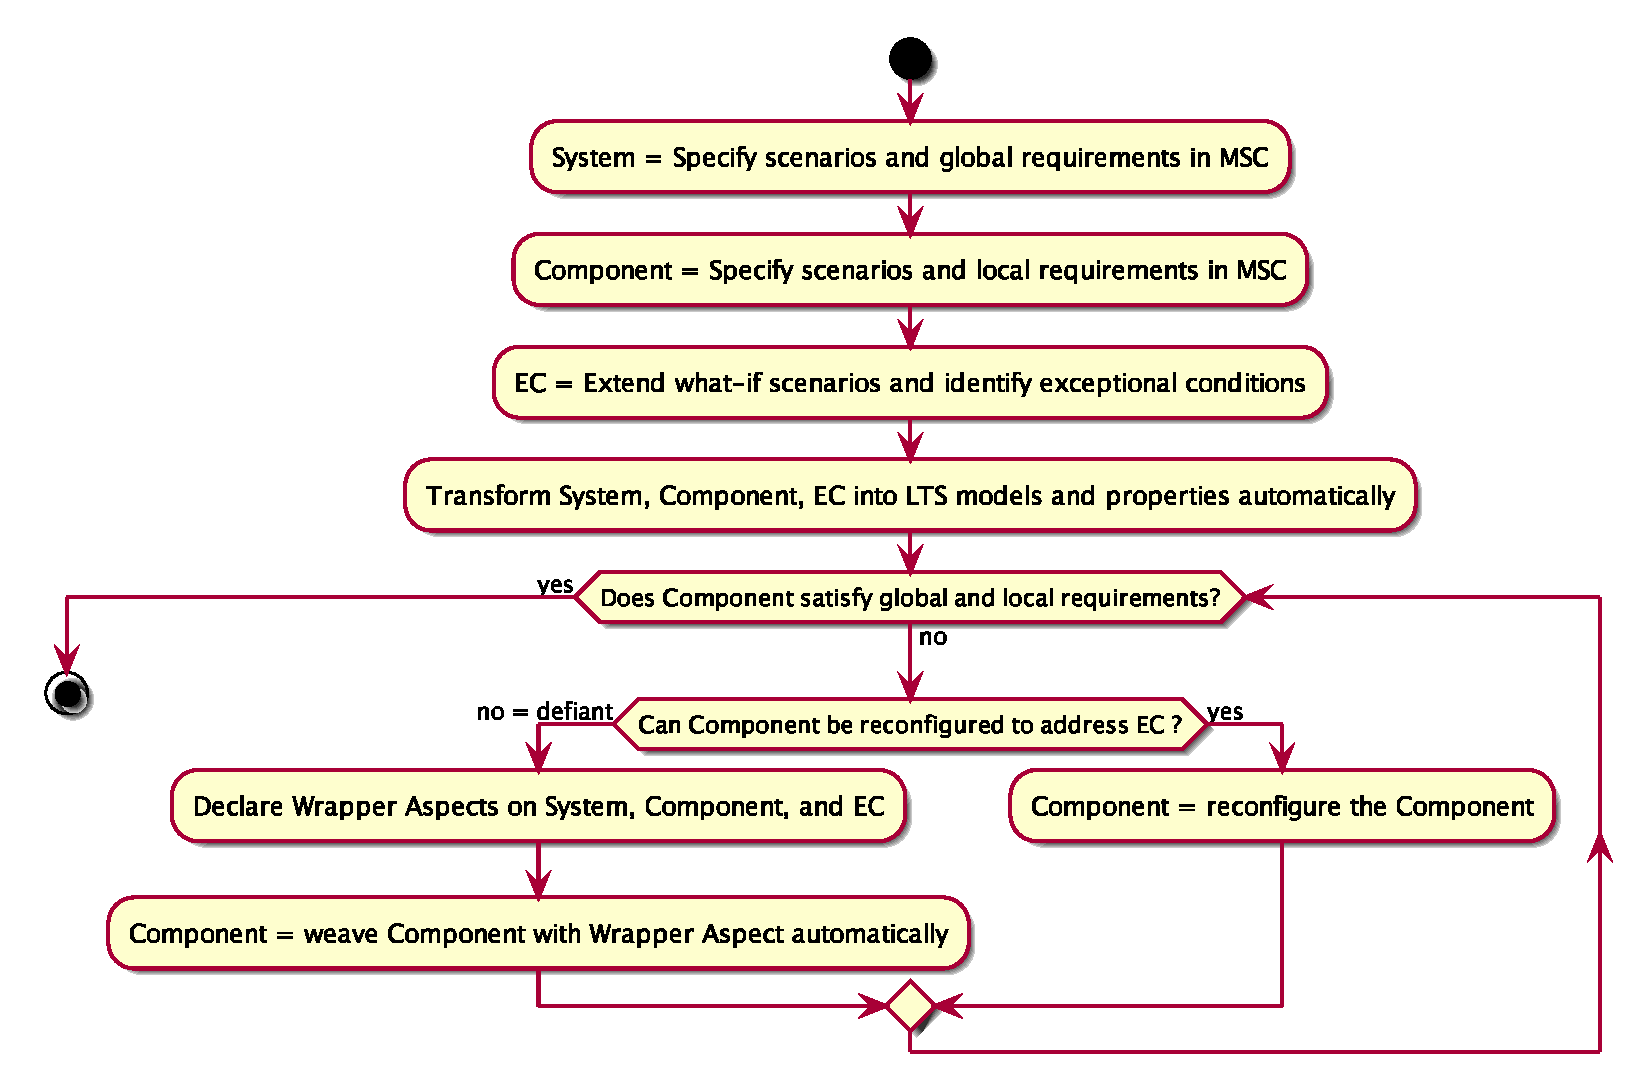
\includegraphics[width=0.9\columnwidth]{figures/activity.eps}
 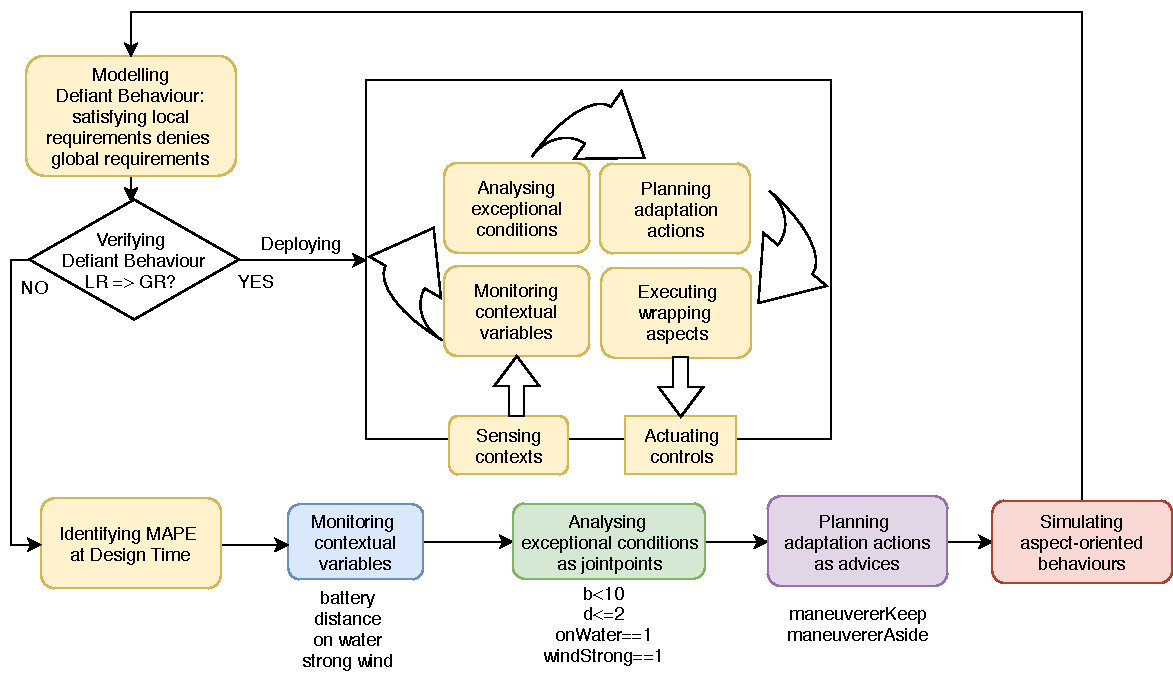
\includegraphics[width=0.8\textwidth]{figures/workflow}
 \caption{Overview of the cautious adaptation approach in a workflow diagram}
 \label{fig:process}
 \vspace*{-0.5cm}
\end{figure*}

%Our approach to cautious adaptation of a defiant component is explained below.

%illustrates the main constructs and relationships between the defiant component and the wrapper framework. The cautious adaptation weaving is responsible of 1) exposing the exceptional conditions of defiant component; 2) identifying the failure of the defiant component under the exceptional conditions; and 3) modifying the functionality of the defiant component to satisfy both exceptional and normal conditions. All these responsibilities can be defined as properties in the behaviour models that can be checked formally. 

%\begin{figure}[ht]
%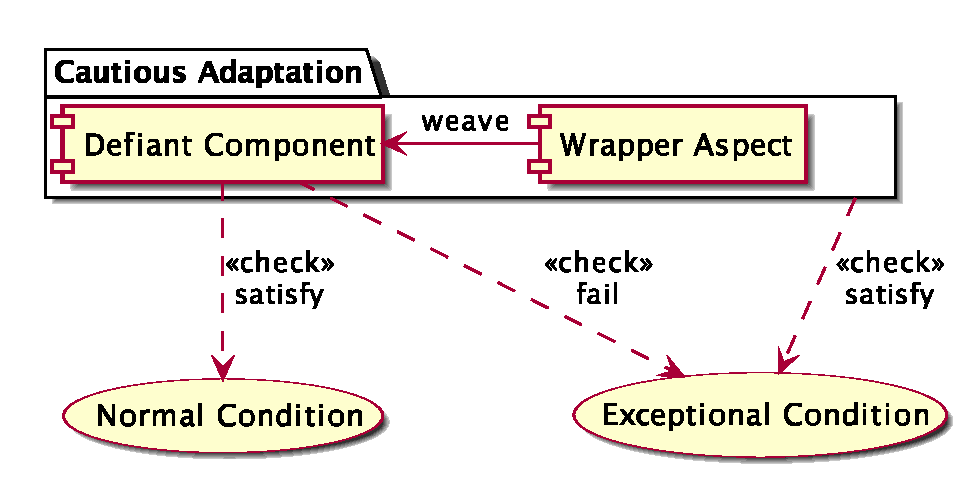
\includegraphics[width=\columnwidth]{figures/overview.eps}
%\caption{Overview of Cautious Adaptation Framework}\label{fig:overview}
%\vspace*{-1cm}
%\end{figure}

\subsection{Formalisation}

The general problem being tackled can be formalised using the semantics of Problem Frames~\cite{DBLP:books/daglib/0022946}, as follows. At the design time of a defiant component ($c$), given its world context ($W_c$), its specification ($S_c$) must satisfy its requirements ($R_c$), i.e., $W_c, S_c \models R_c$. 

%For instance, consider drone component $c$ with two requirements $R_c = R_1 \wedge R_2$, where $R_1$ is ``to fly from location $A$ to location $B$ when the battery level is above a threshold $\theta = 10\%$'' ($W_1$), and $R_2$ is ``to land safely when the battery level drops below $\theta$'' ($W_2 = \neg W_1$).

Suppose that component $c$ is being used as part of a system-of-systems ($s$). Based on the analysis of exception scenarios concerning a specific context of the system ($W_s$), which satisfies the condition $W_s \implies W_c$, component $c$ cannot satisfy global requirements of $s$. In other words, $W_s, S_s \not \models R_s$, where $S_s$ contains $S_c$. 

%In order to illustrate, consider the drone application scenario with an exceptional condition defined as $W_s = W_2 \wedge W_3 \wedge W_4$ where the battery level is below $\theta$ ($W_2$), but the battery level is sufficient to fly to location $B$ because of the wind condition ($W_3$), and it is flying above water by design of $S_s$ ($W_4$). According to the designed specification of the component $S_c$, the drone will land because of $W_2$, regardless of $W_3$, and the drone will land in the water because of $W_4$. The only feasible solution is to avoid safe landing in $W_s$, because if one rescues the landed drone from the water, it will be too late to replace it with another means of transportation even if the payload will not be damaged. Therefore, the problem is that it is not possible to change the specification of $S_c$. 

To verify that the wrapper executes its purpose, we formalise three conditions to be checked as follows:
\[
\begin{array}{ll}
W_s, S_s \not \models R_s & (\mbox{defiant identification})\\
W_s, S_s |_{c\rightarrow w(c)} \models R_s & (\mbox{defiant removal}) \\
W_c \setminus W_s, S_{w(c)} \models R_c & (\mbox{safety assurance})
\end{array}
\]
\begin{itemize}
\item Defiant identification checks that the component is defiant because its configurations do not satisfy global requirements.

\item Defiant removal checks that after wrapping up the defiant component with new behaviour, the global requirement can be restored in exceptional conditions.

\item Safety assurance checks that after wrapping up the defiant component with new behaviour, the local requirements are still satisfied in normal conditions. 
\end{itemize}

\subsection{Scenario Extensions on MSC}
To support the method, we extend the message sequence chart (MSC) specification with an operator (o) to represent an \textit{interception point} in which exceptional scenarios can be plugged to wrap the defiant component. Several exceptional behaviours can be plugged in the same interception point, indicating other possible behaviours according to alternative contexts. If there is no exceptional scenario plugged in an interception point, the expected default behaviour is performed.

Figure~\ref{fig:drone_msc} shows part of high-level message sequence charts (hMSC) specification for the payload organ delivery scenario discussed in Section 1. Each box in the hMSC corresponds to a basic message sequence chart (bMSC), like UML sequence diagrams, exchanging messages between different entities, whilst the bMSC are put together through control flows (branches and loops). Figure~\ref{fig:drone_bmsc} depicts the referred bMSCs for part of the drone payload delivery example.   
% Need one example bMSC. 

\begin{figure}
%    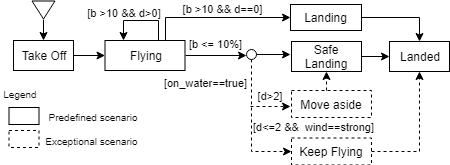
\includegraphics[width=\columnwidth]{figures/new_drone_msc.png}
 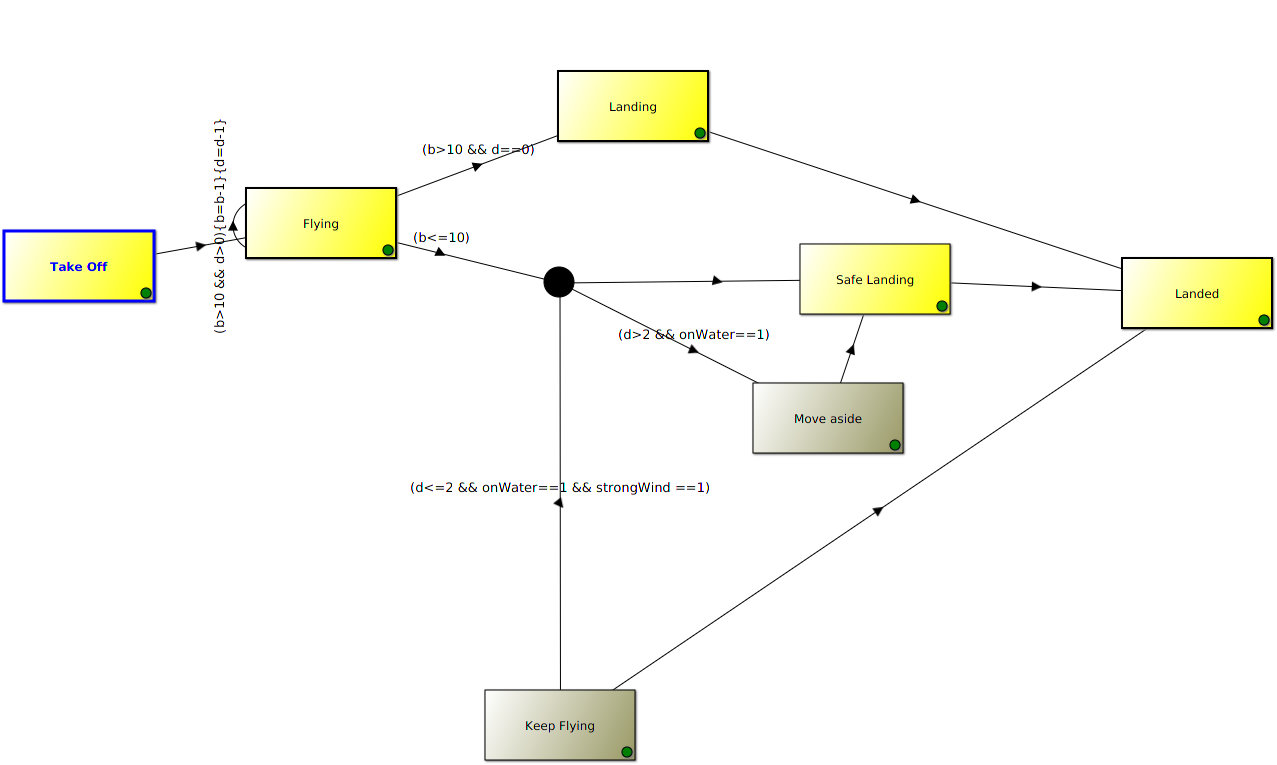
\includegraphics[width=\columnwidth]{figures/1-hMSC-Drone.png}
    \caption{hMSCs for the drone scenario}
    \label{fig:drone_msc}
    \vspace*{-0.25cm}
\end{figure}

\begin{figure}
 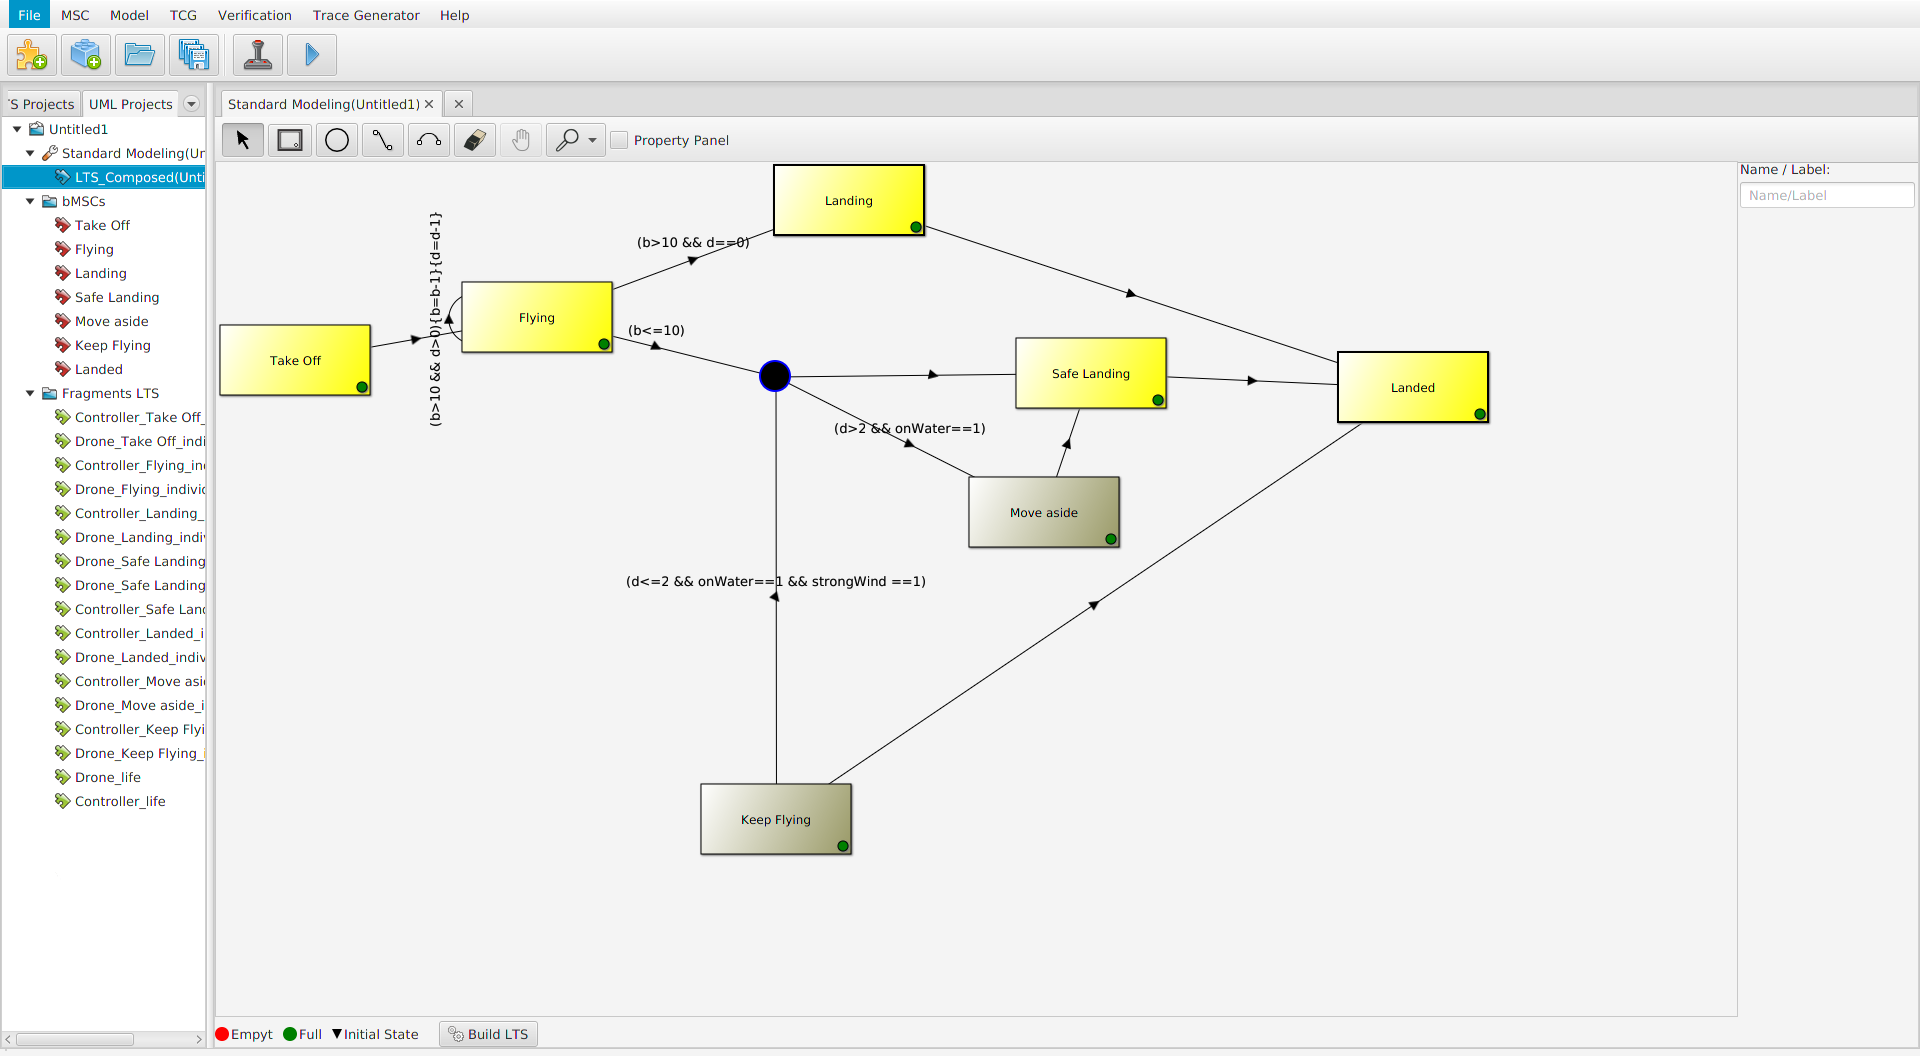
\includegraphics[width=\columnwidth]{figures/2-LoTuS.png}
    \caption{LoTus}
    \label{fig:lotus}
    \vspace*{-0.25cm}
\end{figure}

\begin{figure}
 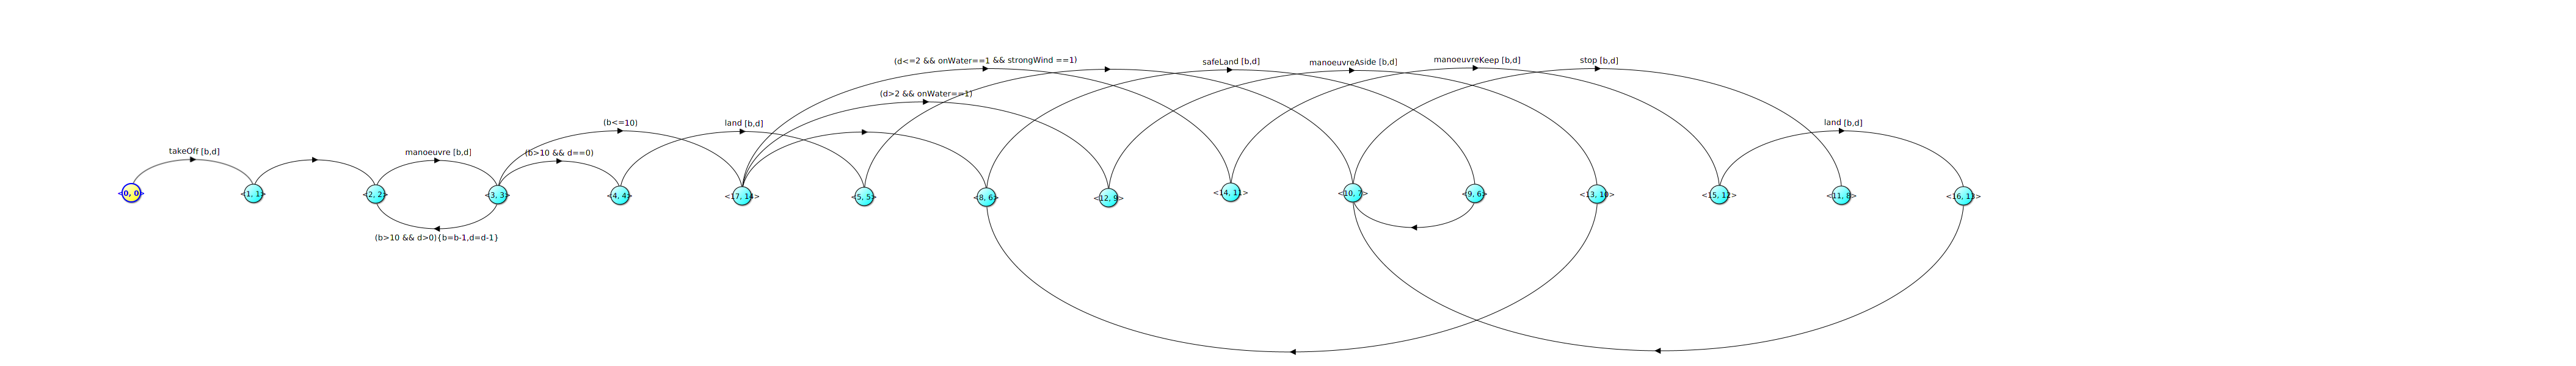
\includegraphics[width=\columnwidth]{figures/3-parameterized-LTS.png}
    \caption{Parameterised LTS}
    \label{fig:pLTS}
    \vspace*{-0.25cm}
\end{figure}

\begin{figure}
 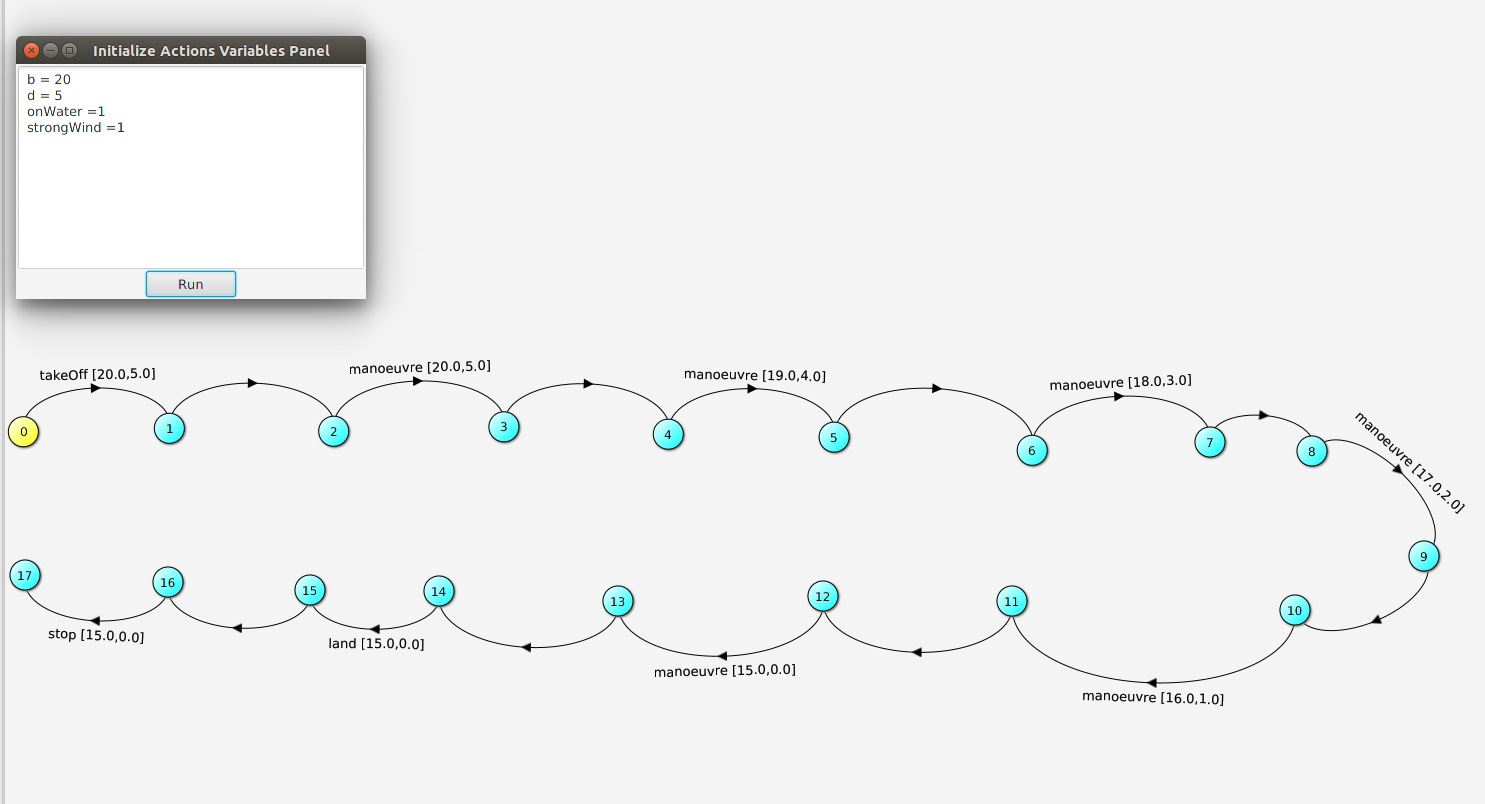
\includegraphics[width=\columnwidth]{figures/4-Land -final-LTS.png}
    \caption{LTS of Landing}
    \label{fig:landing}
    \vspace*{-0.25cm}
\end{figure}

\begin{figure}
 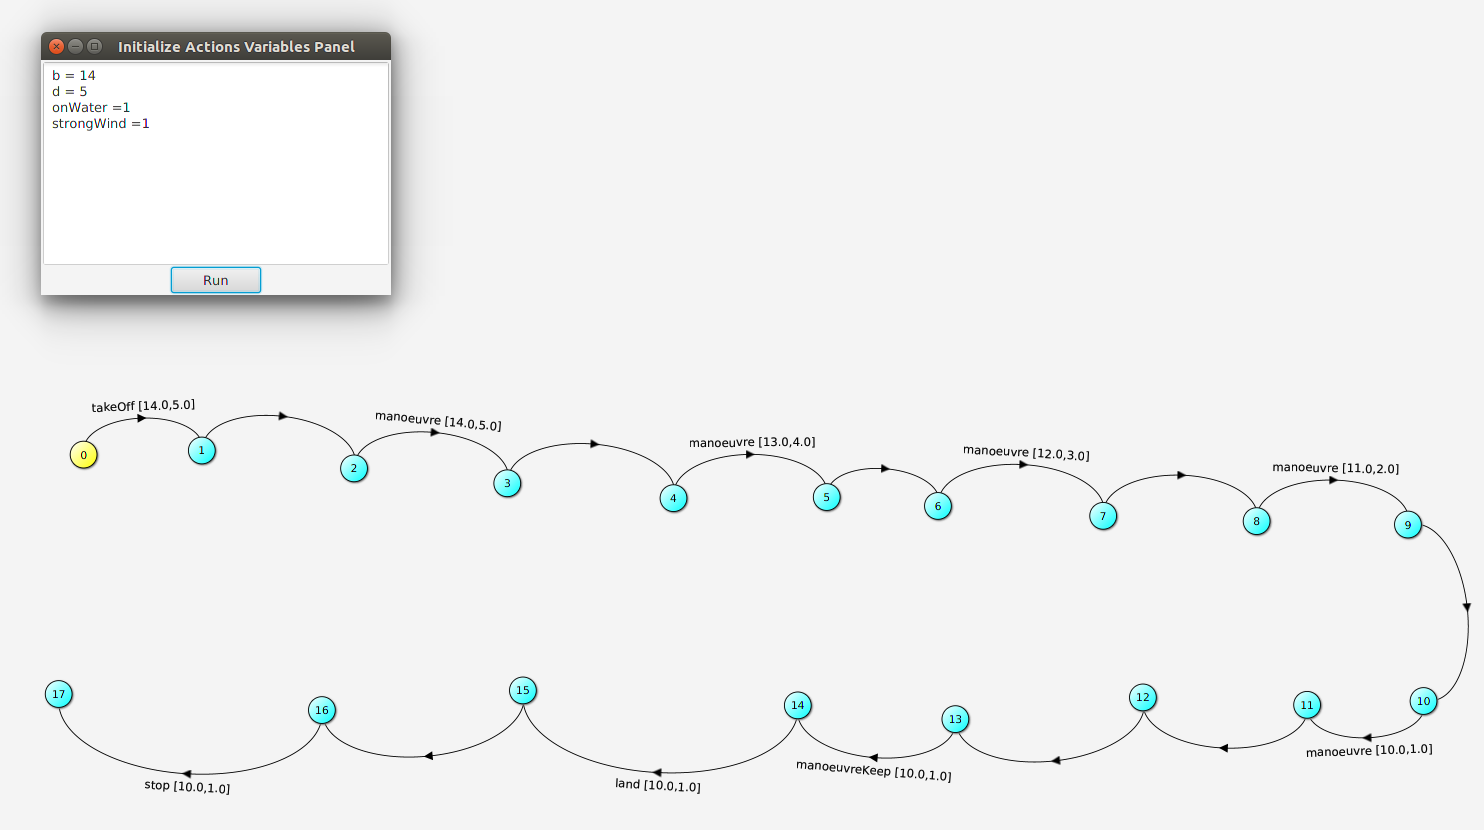
\includegraphics[width=\columnwidth]{figures/5-Keep Flying -final-LTS.png}
    \caption{LTS of Keep Flying}
    \label{fig:keepflying}
    \vspace*{-0.25cm}
\end{figure}

\begin{figure}
 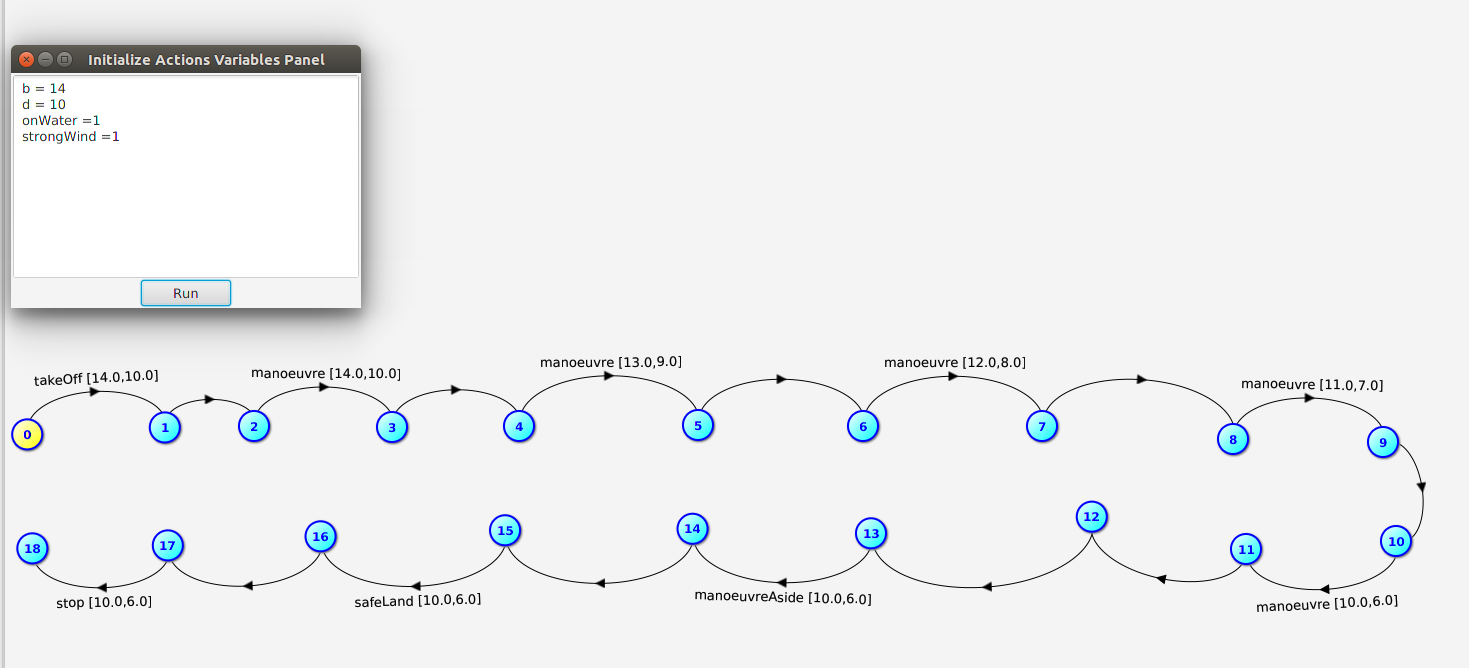
\includegraphics[width=\columnwidth]{figures/6-Move Aside -final-LTS.png}
    \caption{LTS of Moving Aside}
    \label{fig:movingaside}
    \vspace*{-0.25cm}
\end{figure}

%\begin{figure}
%    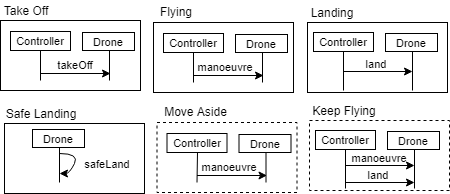
\includegraphics[width=\columnwidth]{figures/new_drone_bmsc.png}
%    \caption{bMSCs for the drone delivery scenario}
%    \label{fig:drone_bmsc}
%    \vspace*{-0.5cm}
%\end{figure}

In Figure~\ref{fig:drone_msc}, the predefined scenarios are represented by a full rectangle and are part of the normal specification of a drone, while the exceptions are represented by dashed rectangles. As shown in Figure~\ref{fig:drone_msc}, through a controller the pilot can control the drone to take off, and can manoeuvre the drone when the battery is above a certain threshold $\theta = 10\%$, while it has not reached the destination. When the pilot sends a landing command to the drone, this is acknowledged when the drone lands in the ground.  During a flight, a drone periodically checks the status of its internal devices such as battery level and distance from the destination, represented by \textit{b} and \textit{d}, respectively, in the guard conditions over the transitions. In the example, if the battery level is above the expected threshold and the drone is not yet in its destination, the drone keeps flying. If the drone reaches its destination, it performs a landing action. If the battery is below the expected threshold, the drone performs a safe landing in accordance to its predefined specification. 

The exceptional conditions added in the interception point state that if the distance to the expected destination is less than 2km, the drone is flying over the river (condition \textit{on\_water==true}), and the wind is strong (condition \textit{wind==strong}), then the pilot can keep the drone flying even in a low-level battery situation and then land, thus being able to complete its overall goal (delivering the medical payload) successfully. Nonetheless, if the battery is low, the drone is above water, but the drone is more than 2km away or the wind is not strong,
% Paolo: Fig 2 needs update
% "[d > 2]" => "[d > 2 || wind!=strong]"
then the action is to move the drone aside in order to land it on the ground. 

% Figure~\ref{fig:overview} shows an overview of the relationship between the defiant component and the wrapper technique. The cautious adaptation approach is responsible to: (i) expose exceptional conditions of defiant components; (ii) identify failure of  defiant components under the exceptional conditions; and (iii) modify the functionality of defiant components to satisfy both exceptional and normal conditions. All these responsibilities can be defined as properties in behaviour models that can be checked formally. 

\subsection{The Wrapper Aspect}
The introduction of a {\it wrapper} $w(c)$ changes the defiant behaviour of the component $c$, i.e. $W_s, S_{w(c)} \not \models R_c$, retaining the essential satisfaction of global requirements when $c$ is substituted with $w(c)$:  $W_s, S'_s \models R_s$ where $S'_s = S_s |_{c \rightarrow w(c)}$. Furthermore, the adaptation is {\it cautious} because other than the exceptional condition $W_s$, the wrapped component should still behave like the original designed component, i.e., $(W_c \setminus W_s), S_{w(c)} \models R_c$. 

%\subsubsection{A Wrapper by Aspect-Orientation}
Based on aspect-oriented programming (AOP)~\cite{Kiczales:2001}, we introduce wrappers that can achieve the above requirements. The exceptional conditions identified in the scenarios provide an indication where changes in the system should occur ({\it joint points}). Once the join points are identified, we represent them as regular expressions as {\it point-cuts}, so that a replacement of the behaviour after the join points can be done through aspect {\it advices}. Aspect advices are exceptionally handled, which can invoke existing functionalities of original components, but can also introduce additional functions and conditions that do not exist in the original components.

%Since a component at design time is unaware of its future exceptional usage, it will not be able to expose its full implementation to the system integrator. Fortunately, {\it aspect-oriented} framework can intercept the control flow of the behavioural specification~\cite{Xu07}. 

%For example, to identify the join points, i.e., where  modifications are allowed to change. Methodologically, the exceptional conditions we obtain from the exceptional scenarios provide us a clue where such join points can be.

%Once the join points are identified, we can use regular expressions to express them as {\it point-cuts} so that a replacement of the behaviour after the join points can be done through aspect {\it advices}. Aspect advices in this situation are exceptional handling which can still invoke existing functionality of the original components, but can also introduce additional functions and conditions that do not exist in the original component. But the weaving of the aspect-oriented wrapper must be performed with caution. 

In the situation in which there are more than one wrapper for the same exceptional condition, to avoid interference~\cite{Katz:2008:IAI:1394496.1394500}, we define a precedence order among wrappers. For example, a safety wrapper is regarded with a high-level of importance and should be applied afterwards, to override applied unsafe wrappers. 

\subsection{Discussion about Self-Adaptation}

Existing self-adaptive systems rely on a full monitoring-analysis-planning-execution (MAPE) feedback loop to continuously monitor the environment and switch to alternative solutions when the requirements are not satisfied.
However, we observe that it is not always necessary to monitor the entire process. Given the prior knowledge of the environment, to reduce the monitoring and adaptation overhead, it is possible to monitor only part of the processes while switch to part of the solutions when the adaptation is required. 
In this way, cautious adaption can be seen as a means towards more efficient self-adaptation.

TODO. Can we evaluate the efficiency of self-adaptation by measuring the efficiency?
\section{Detailed Process}

In this section each phase of the proposed approach is detailed using the running example introduced in the previous section.

\subsubsection{Defiant component identification}

% First step: Modelling normal scenarios 
Initially, we use scenarios to model the core functional requirements for the self-adaptive system and the local requirements for each component. Scenarios formalise both exceptional and normal conditions of the system, which have been widely used for modelling {\it what-if} situations~\cite{Uchitel2003}. It assumes the use of off-the-shelf software components, with predefined requirements and specifications. 

Figure~\ref{fig:drone_msc} shows part of hMSC specification for the payload organ delivery scenario discussed in Section 1. Each box in the hMSC corresponds to a basic message sequence chart (bMSC), exchanging messages between different entities, whilst the bMSC are put together through control flows (branches and loops). Figure~\ref{fig:drone_bmsc} depicts the referred bMSCs for part of the drone payload delivery example.

\begin{figure}
    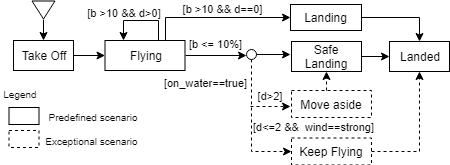
\includegraphics[width=\columnwidth]{figures/new_drone_msc.png}
    \caption{hMSCs for the drone scenario}
    \label{fig:drone_msc}
    \vspace*{-0.25cm}
\end{figure}

\begin{figure}
    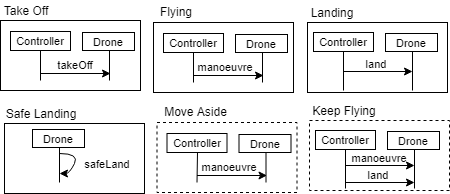
\includegraphics[width=\columnwidth]{figures/new_drone_bmsc.png}
    \caption{bMSCs for the drone delivery scenario}
    \label{fig:drone_bmsc}
    \vspace*{-0.5cm}
\end{figure}

In Figure~\ref{fig:drone_msc}, the predefined scenarios are represented by a full rectangle and are part of the normal specification of a drone, while the exceptions are represented by dashed rectangles. As shown in Figure~\ref{fig:drone_msc}, through a controller the pilot can control the drone to take off, and can manoeuvre the drone when the battery is above a certain threshold $\theta = 10\%$, while it has not reached the destination. When the pilot sends a landing command to the drone, this is acknowledged when the drone lands in the ground.  During a flight, a drone periodically checks the status of its internal devices such as battery level and distance from the destination, represented by \textit{b} and \textit{d}, respectively, in the guard conditions over the transitions. In the example, if the battery level is above the expected threshold and the drone is not yet in its destination, the drone keeps flying. If the drone reaches its destination, it performs a landing action. If the battery is below the expected threshold, the drone performs a safe landing in accordance to its predefined specification. 

% Second step: extend the MSC with exception scenarios
The second step consists of extending the initial scenario specification with the identified exceptional scenarios and context variables. Here we augment the MSC specification with an interception point, that represents the moment on which a condition is analysed in order to decide whether the original expected scenario is executed or an introduced exceptional scenario has to take place instead. 

The exceptional conditions added in the interception point state that if the distance to the expected destination is less than 2km, the drone is flying over the river (condition \textit{on\_water==true}), and the wind is strong (condition \textit{wind==strong}), then the pilot can keep the drone flying even in a low-level battery situation and then land, thus being able to complete its overall goal (delivering the medical payload) successfully. Nonetheless, if the battery is low, the drone is above water, but the drone is more than 2km away or the wind is not strong, then the action is to move the drone aside in order to land it on the ground.

% Paolo: Fig 2 needs update
% "[d > 2]" => "[d > 2 || wind!=strong]"

% Third step: generate the parameterized LTS
Subsequently, the complete MSC scenario specification is automatically transformed to a parameterized Labelled Transition System (LTS), which contains in the scenario transition conditions as guards in the corresponding state transitions that represent the scenario change. The reason for converting scenarios into LTS formally is to facilitate the correctness checks of the model before and after the adaptation. %The scenarios representing the system (with the off-the-shelf components) are transformed into LTS behaviour models, and requirements are transformed into properties. 

The MSC-to-LTS generation algorithm is an adaptation of the one proposed in ~\cite{Rodrigues:2005}, with the introduction of the scenario transition guards in the resulting LTS. Figure~\cite{fig:pLTS} depicts the parameterized LTS generated for the drone example of Figure 1. 

\begin{figure*}\centering
 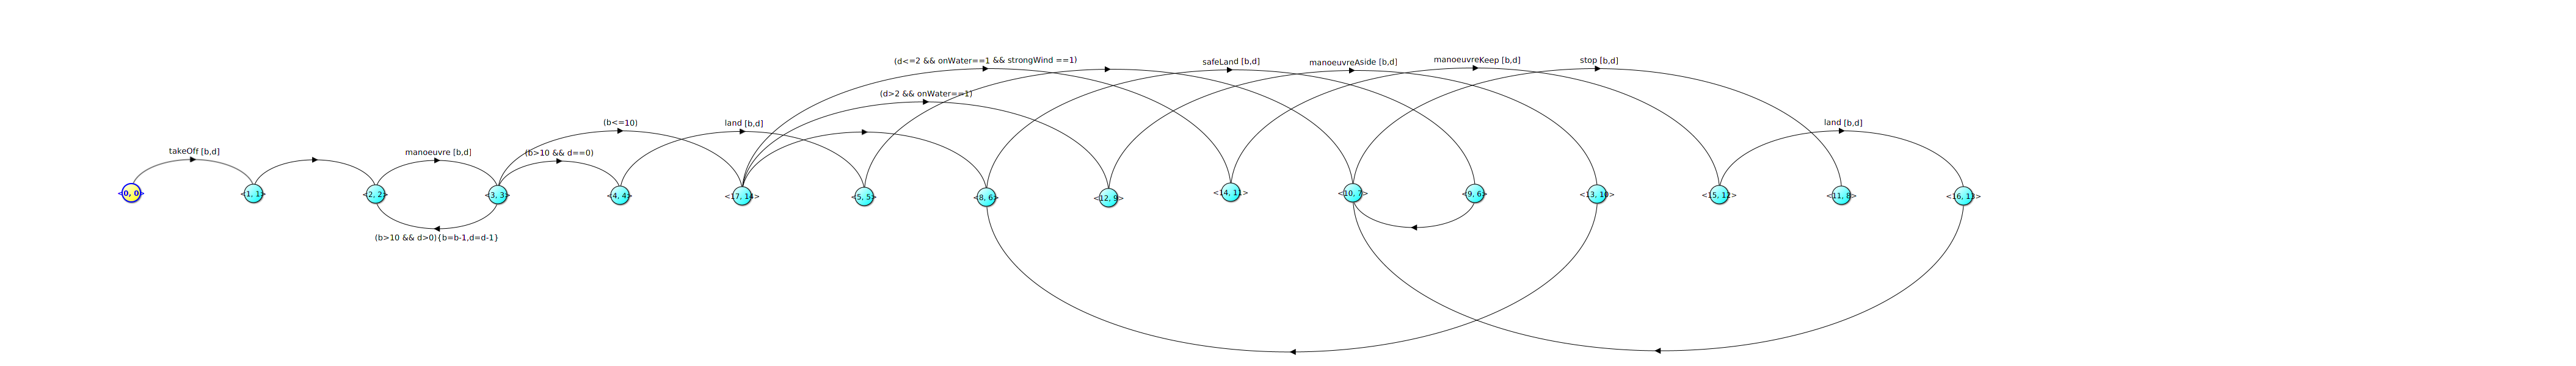
\includegraphics[width=\textwidth]{figures/3-parameterized-LTS.png}
    \caption{Parameterised LTS illustrates the behaviours when the contextual variables are parameters bound to user specified constants. }
    \label{fig:pLTS}
    \vspace*{-0.25cm}
\end{figure*}

%Given the similarities between exceptional and what-if conditions, the approach uses existing formal method techniques, like feedback-driven implied scenario resolutions~\cite{uchitel:2013}, to verify scenarios represented as message sequence charts (MSC) translated into labelled transition systems (LTS), with respect to safety and liveness properties. 
%\textbf{Note: we need a justification here!}

%Fourth step: generation of final LTS 
After that, the user can set the values of the context variables and instanciate a context-specific LTS.

\begin{figure*}\centering
 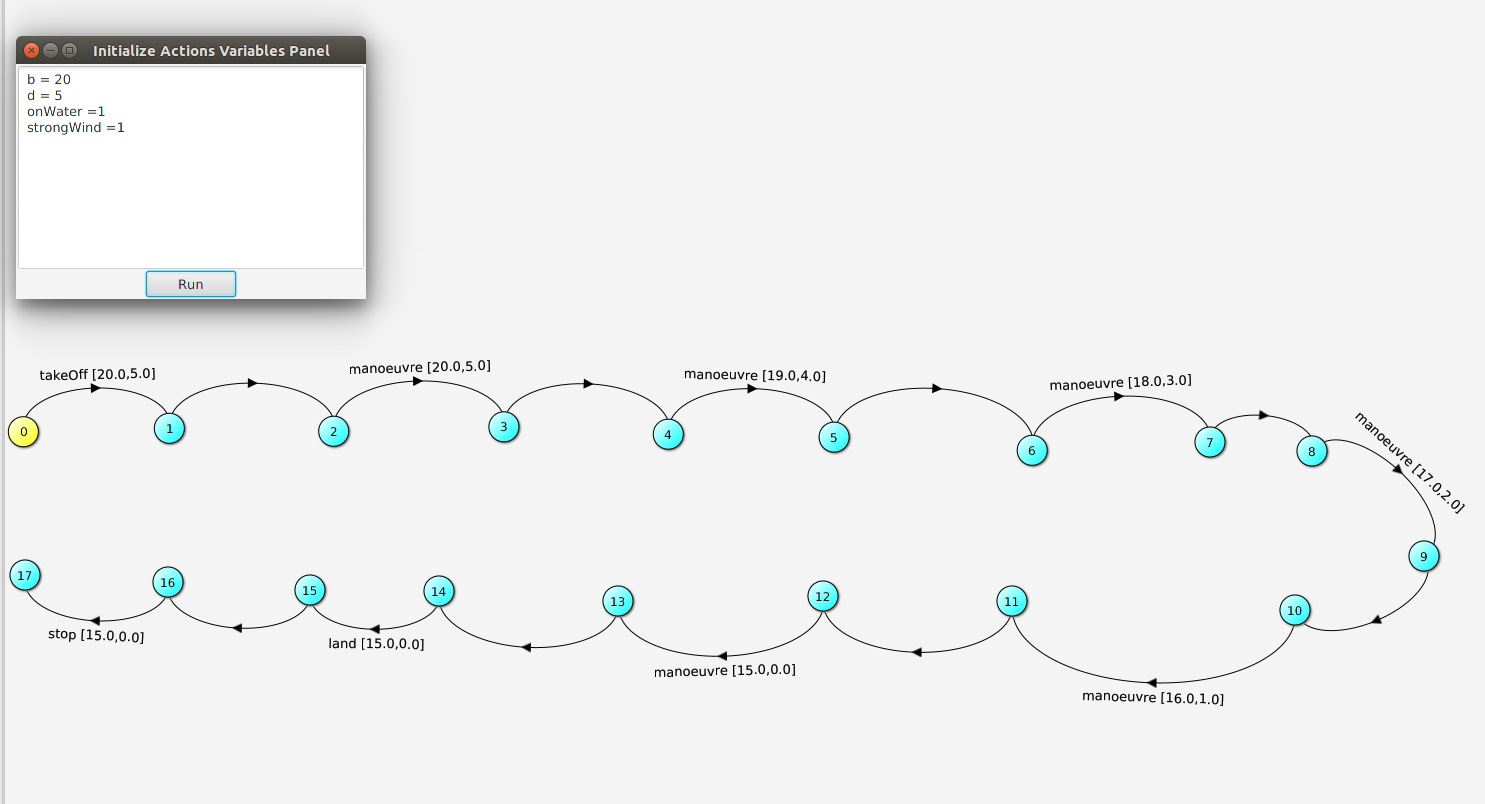
\includegraphics[width=0.8\textwidth]{figures/4-Land-final-LTS.png}
    \caption{LTS of Landing: the partial behaviour of landing bMSC, where the unnamed transitions are the transitions between different bMSCs. Though an $\epsilon$-reduction, these transitions will be removed.}
    \label{fig:landing}
    \vspace*{-0.25cm}
\end{figure*}

%Fifth step: checking local and global requirements
That LTS can be exported to LTSA in order to check both local and global requirement specified in terms of properties. If the generated behaviour satisfies local requirements but does not satisfy the global ones, then a defiant behaviour is identified and has to addressed, otherwise the component can be used as it is in the new system of system.
The verification of the satisfaction arguments of global requirements and local requirements provides designer a formal basis to tell whether or not defiant behaviour exists in the components, and whether or not addressing the defiant behaviours (i.e., an off-the-shelf component cannot satisfy the global requirements out of the box). 

If the identified defiant component can be reconfigured (for instance, via source code alteration or parameterization), then a component reconfiguration occurs. This is out of scope of this research. After that, the new component behaviour is verified again in order to check whether it satisfies the local and global requirements. 

A model checker is applied to verify whether the off-the-shelf component can also satisfy  global requirements of the system-of-system, for which not necessarily it was designed. In the case when the component satisfies the requirements, it can be used as-is in the system-of-system. However, when the component cannot be changed (i.e., the case of a defiant component), a wrapper is specified in order to weave exceptional conditions into the component specification in LTS, and it is verified by the LTSA model checker against the properties.  The adaptation is considered {\it cautious} only when {\bf all} the properties (local and global) are satisfied by the component within the system-of-system context. The verification step is considered successful, that is, the defiant behaviours can be addressed by design-time simulation and verifications. 

\subsubsection{Wrapper Design and Implementation}

In the first step, contextual variables for analysing the global requirements are elicited such as battery levels, distance to destination, drone is over the water or not, and whether or not the wind is favorable, etc.  These variables may not be available or used for analysing the local requirements of the component. Nonetheless, from a bigger picture, usually they are critical to tell the satisfaction of the global requirements. 

The second step aims at analysing situations when the satisfaction of local requirements denies the satisfaction of global requirements in order to identify the exceptional conditions. The what-if situations marks exceptional conditions on an extension of the scenario models, which will also be transformed into safety properties in LTS.  E.g., battery level is lower than 10\%, distance to destination is smaller than 2km, the drone is over the water, and the wind is favourable to cover the remaining distance with fewer power. The combination of these conditions would trigger a situation that it is in fact possible to satisfy the global requirements by the drone, only if some of its existing safety assumption is updated. In the opposite case, the failed checks are used to identify how to deal with exceptional conditions. %From the counter examples provided by the model checker (i.e., sequences of actions that lead to failures), software designers can inspect which of the actions can be avoided by negating the conditions that trigger these action in the behavioural model. These triggered conditions are combined to form exceptional conditions. The negation of an exceptional condition is considered as a normal condition.

In the next step, the exceptions can be addressed by Planning adaptation actions in the component. Using the existing functionalities such as maneuveuring, while disabling certain functionaties such as safe landing, it is possible to switch to a different solution through adaptation. Such adaptions are modelled as advices such as before / around of existing functionalities/actions in the adapted component.

\item {\bf Simulating circumventing behaviours.} Under exceptional conditions the alternative adaptation actions need to be called, however, the existing component is not designed to be adaptable. In this step we uses aspect-oriented mechanisms to weave the changes into the system behaviours and pass the modified behavioural model back to the verification step. Note that this step is still performed at the design time, therefore we cannot call it ``execution", but it is corresponding to the execution step of the MAPE self-adaptive system at the runtime.

After the wrapper has been implemented, the last step consists on deploying it on the system so it can adapt at runtime the behaviour of the defiant components.

\subsubsection{Runtime Cautious Adaptation}

Here comes the text... 
\section{Implementation and Evaluation}

In this section we present how we evaluated our approach. To do that, we extended the drone example with following scenarios, as illustrated by Figure~\ref{fig:simulation-scenario}: 

\begin{itemize}
    \item return to home/gliding: the return-to-home feature is executed whenever the drone bypasses a bad connection area (for instance, near to communication towers) in which the the drone loses connection with the pilot. This is a common safe procedure present in most drones currently. In the case of the medical payload delivery, this safety component becomes defiant since the bad connection can be transient and the drone could glide while waiting for the connection return. This way, we can maximize the chance of delivering the payload.  
    \item economy mode: if the battery reaches 15\%, then the drone enters in the economy mode, in which same sensors and the camera are switched off in order to save battery. However, by doing this, the pilot can loses the control of the drone, which may put in risk the medical payload. Therefore, the economy mode becomes defiant and should not occur during the medical delivery mission. 
\end{itemize}

\begin{figure*}[h]\centering
% 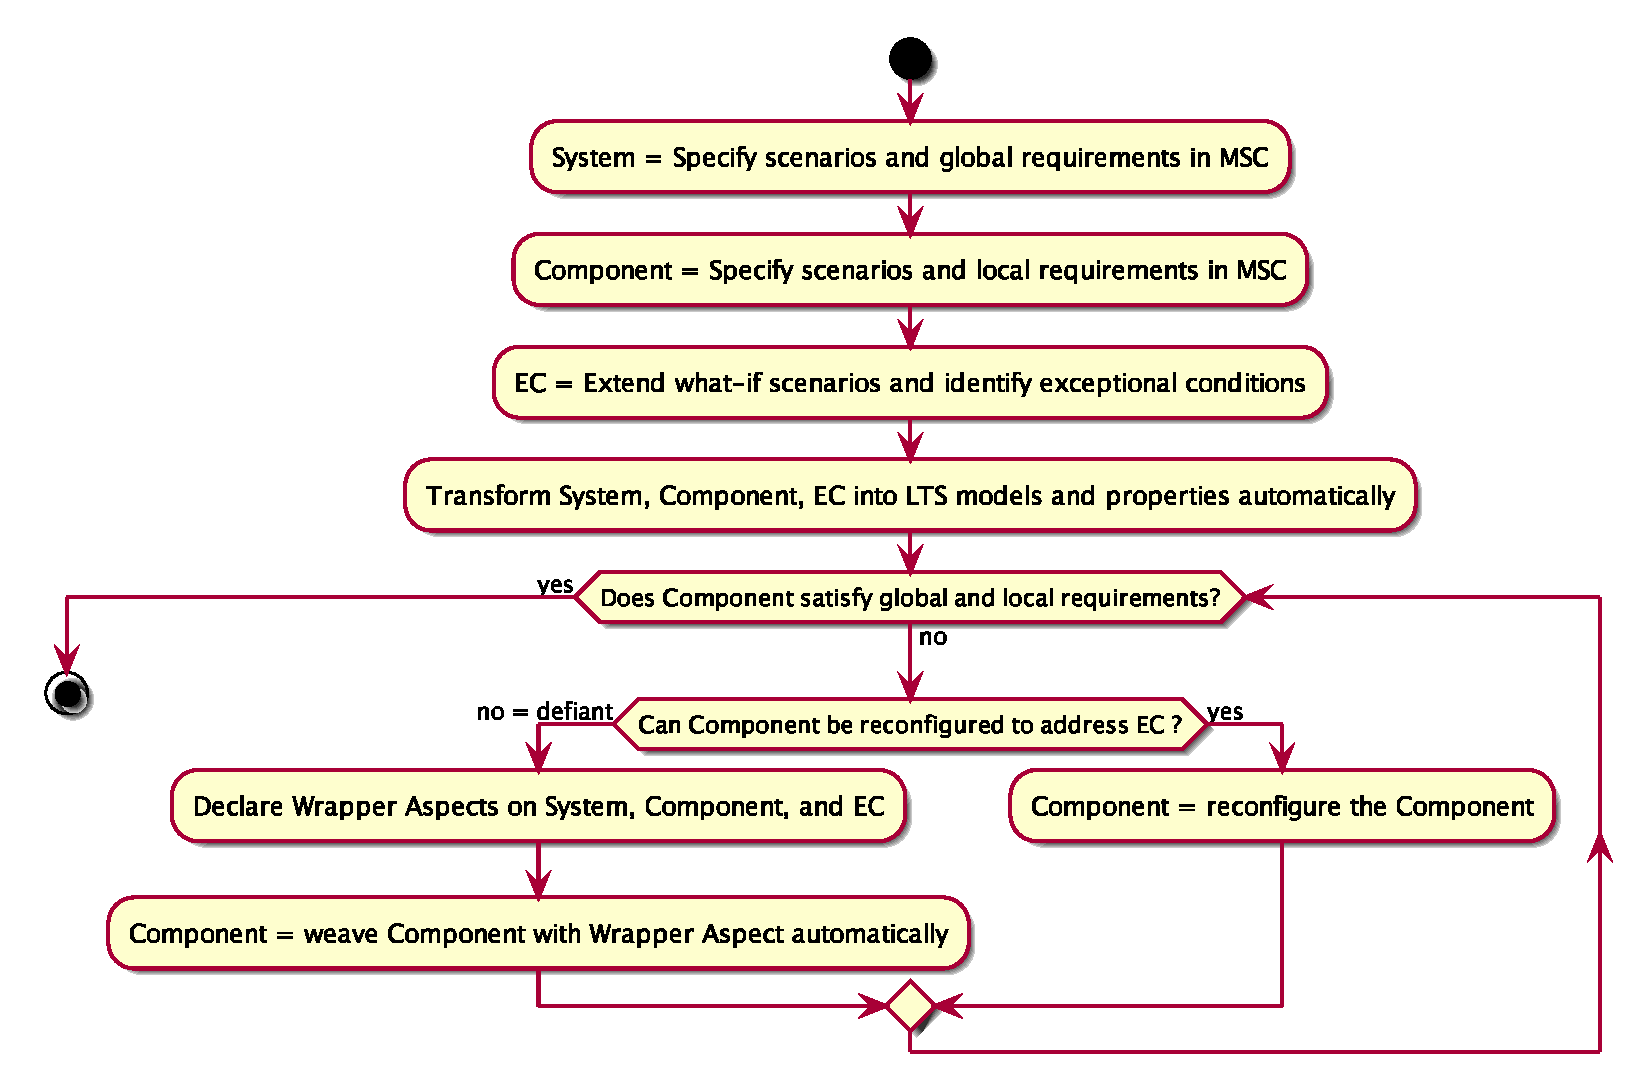
\includegraphics[width=0.9\columnwidth]{figures/activity.eps}
 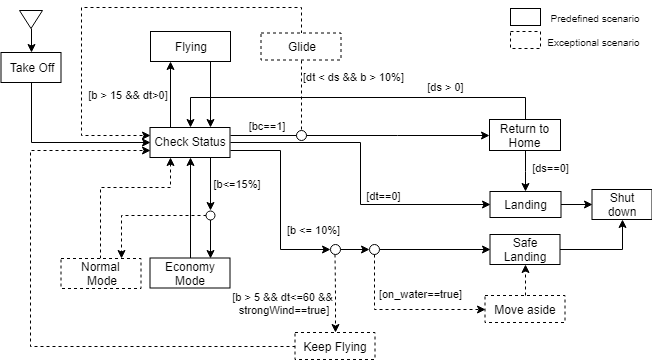
\includegraphics[width=0.7\textwidth]{figures/simulation-scenario.png}
 \caption{Simulation scenario}
 \label{fig:simulation-scenario}
 \vspace*{-0.5cm}
\end{figure*}

We implemented a prototype that simulates all behaviours indicated in Figure~\ref{fig:simulation-scenario}. Then we implemented a wrapper following the proposed approach described in section 3.1. In the simulator, the user can control either one or several drones at the same time. He/she can insert in a graphical user interface the source and destiny hospital, the communication towers, and draw the shape of the river. A snapshot of the simulator is depicted by Figure~\ref{fig:simulator}.   

\begin{figure}[h]\centering
% 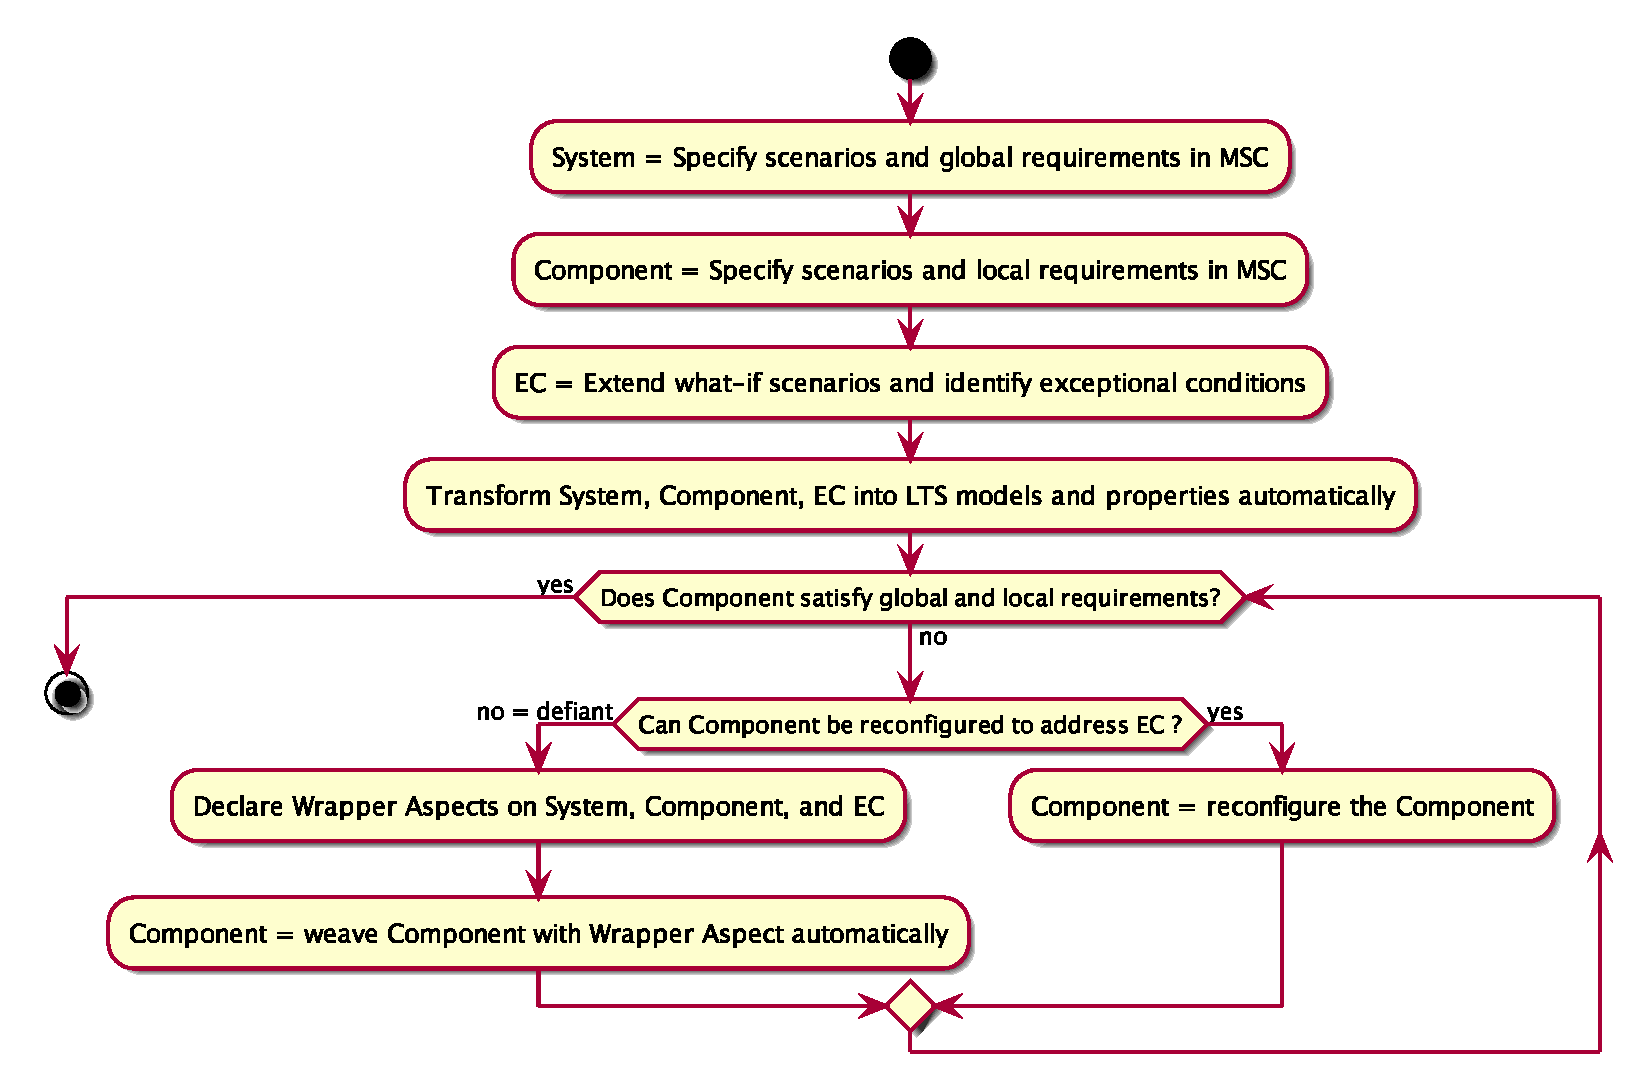
\includegraphics[width=0.9\columnwidth]{figures/activity.eps}
 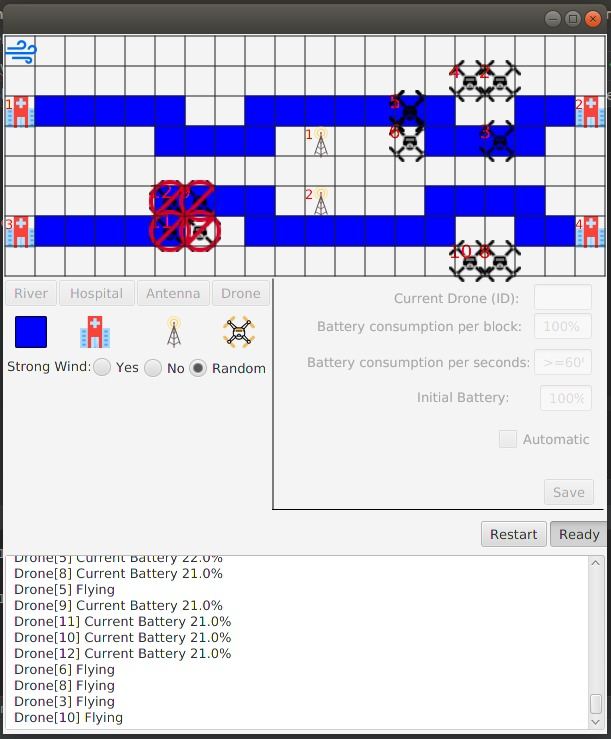
\includegraphics[width=0.4\textwidth]{figures/simulation.jpg}
 \caption{Screenshot of the simulation prototype}
 \label{fig:simulator}
 \vspace*{-0.5cm}
\end{figure}

We considered three criteria: (i) \textit{defiance removal}, which regards whether the drone behaves as expected with the wrapper; (ii) \textit{effectiveness}, regards when a fleet of drones is used to accomplish a mission; and (iii) conflict resolution, in which we discuss how our solution deals with when two or more components turn defiant at the same time. Each criterion is discussed as follows.

\subsection{Defiance removal}

Text to come...

\subsection{Effectiveness}

Text to come...

\subsection{Conflict resolution}

Text to come...



% \section{Related work}

% In ~\cite{John:2004} the authors propose an agent‐ based modeling for capturing and identifying and assessing emergent behaviours in SoS... 

% In ~\cite{Wachholder:2015}, the authors propose modeling emergent behaviour in a SoS using bigraph...

% Mittal and Cane describe various qualitative knowledge engineering methodologies that can be used to close the knowledge-gap for strong emergent behavior and add contextualization with system-of-systems overall purpose so that modeling and simulation can be applied in systems engineering life cycle for reproducible and predictable SoS emergent behavior ~\cite{Mittal:2016} 

%%In ~\cite{Braberman:2015} the authors propose MORPH, a reference architecture...

%%In ~\cite{Zhang:2017}, a self-adaptive distributed decision support model for IoT applications is proposed. The model has been designed using an artificial neural network (ANN) for environment recognition, a knowledge merging to create a local knowledge base and an expert systems for decision making that finally provide intelligent support for IoT applications. However, the proposed model does not deal with conflict of interests of system components at runtime. 

\section{Conclusion and Future Work}

% Generalise the problem
%Although we have only described two possible scenarios, 
%The {\em defiant} problem may happen to various applications including cyber-physical systems, service-based systems, cyber security, system of systems, and cloud computing. The problem is challenging to predict at design time since each component has only local awareness of the system, restricted to its own behaviour model. However, when the components interact with each other at runtime, a global awareness of the system is needed where the interaction among the components cannot be anticipated at design time, due to the unpredictable human behaviour, possible component failures or on-the-fly intercommunication between a highly inter-operable and decoupled systems. Furthermore, the decisions about system conflict resolutions have been taken at design time.   


In this paper we have proposed a novel approach to address the problem of components that were not developed to be adapted during their execution,  but which must then participate in a system-of-systems that does requires them to adapt . We called these components {\it defiant}. Our approach supports what we call  {\it cautious} adaptation, in which wrappers are used to  deal with exceptional conditions. These wrappers specify how the components should behave in case of exceptional conditions. They are woven into the components, and our approach guarantees the satisfaction of both normal and exceptional conditions. The exceptional conditions are identified from the counter examples provided by a model checker when verifying properties of the system-of-systems in which the components participate. To illustrate the work, we use an example of a drone payload organ delivery application.

Currently, we are extending the approach to support on-the-fly identification of new exceptional conditions due to emergent behaviours and their respective wrappers. We are also evaluating the work in other large-scale scenarios.


%Unlike traditional adaptation or self-adaptation approaches, the cautious adaptation makes no assumption that the defiant component can be changed directly. Instead, its functionality needs to be maintained for the normal condition, and only modified when the exceptional conditions are identified in the what-if scenarios. Furthermore, the actions of the defiant component required to fulfill the exceptional conditions also need to satisfy their new expectations, which may not be automatically satisfied by their original design.

%Using an illustrative example, we have verified the wrapper aspect through a model checker against several cautious adaptation conditions. In the future, we will implement the wrapper aspects for large-scale examples.



\bibliographystyle{IEEEtran}
\bibliography{references}

\end{document}
